\chapter{Strings: Multi-tenancy in Accelerator-based Servers}

%\section{Introduction}
Cloud and server infrastructures routinely use GPUs to service computationally intensive client workloads, for online gaming~\cite{nvidia-game}, multimedia services~\cite{element} and image processing~\cite{adobe}, financial codes~\cite{zillians}, data mining~\cite{GPUmine} and search~\cite{GPUsearch}, and to support the needs of next generation applications like perceptual computing~\cite{GPU29, GPU30, GPU31, GPU32, GPU33}. This trend is mirrored by GPU offerings by cloud providers like Amazon ECC~\cite{amazon}, Nimbix~\cite{nimbix}, Peer1 Hosting~\cite{peer1}, and Penguin Computing~\cite{penguin}. 

The effective use of GPUs in these multi-tenant server and cloud infrastructures, however, challenges the current model of static GPU provisioning, in which applications explicitly and programmatically select the GPU devices on which they wish to run. Such static GPU assignments will inhibit concurrency, particularly with the varying workloads imposed by web applications. For instance, during peak demands for certain services, their GPU devices will be heavily utilized while other services' GPUs will be idle or underutilized. Additional GPU underutilization will be caused by application-specific variations in their fraction of CPU vs. GPU execution time, for reasons that include an inability to parallelize certain application components and/or limited GPU residency vs. the costs of host-GPU data transfers.

The \textit{Strings} scheduler described in this chapter adopts a multi-tenant model in which accelerators like GPUs are treated as first class schedulable entities~\cite{gdev, gvim, ravi, pegasus}, by overriding the device selection calls made by applications and then managing their GPU calls with a two-level scheduler: at the higher level, on each platform, balancing workloads across the multiple GPUs attached, and at the GPU device level, reducing core idling via multi-tenancy and the judicious overlap of GPU execution with host-GPU data movements. Additional performance improvements are derived from dynamically merging the GPU contexts of different applications and by providing dynamic feedback about fine-grain application characteristics from device-level schedulers to the workload balancer.

Using \textit{Strings} with workloads drawn from diverse classes of cloud applications, this chapter presents and evaluates GPU scheduling policies distinct from prior work in their explicit consideration of data movement to/from the GPU device. (1) The Phase Selection (PS) policy co-schedules on the same GPU those applications that currently operate in different phases – computation vs. communication -- of their combined CPU/GPU execution. Using PS results in an average speedup of \textbf{6.41x} over static provisioning with the CUDA runtime. (2) Advanced feedback-based policies, termed Data Transfer Feedback (DTF) and Memory Bandwidth Feedback (MBF), capitalize on the advantages offered by CUDA streams and by Strings’ built-in support for merging GPU contexts belonging to different applications. DTF collocates applications with contrasting data transfer times to maximize the concurrent use of a GPU's memcpy vs. compute engines. MBF improves overall performance by concurrently executing and hiding the large memory latencies seen by a memory bound application by switching to a compute bound application. DTF and MBF achieve notable improvements in average system throughput, by \textbf{8.06x} and \textbf{8.70x}, respectively, compared to the commonly used CUDA runtime. (3) Further improvements in performance are derived from dynamic changes to the workload balancing policies being used in response to device-level observations of altered behavior in the GPU tasks being run.


This chapter makes following technical contributions:
\begin{itemize}
\item A two-level hierarchical scheduler where workload balancing intelligently binds each application’s GPU component to an appropriate GPU, along with a device- level, per-GPU scheduler that handles GPU resource sharing for the multiple tenants mapped to a single GPU, to improve application performance while also meeting system-level goals like high throughput, fairness, etc.
\item Support for multi-tenancy, termed the Context Packer, which dynamically packs the GPU contexts of multiple applications into a single context, to achieve high GPU utilization and low context switching overhead.
\item Dynamic feedback from device-level schedulers to workload balancer, to inform the global decisions made by the latter about the characteristics of the applications being scheduled by the former.
\item A novel GPU scheduling policy, called Phase selection (PS), which maximizes the concurrent use of a GPU’s memcpy vs. compute engines, by smartly selecting applications currently running in different phases of their combined CPU/GPU execution.
\item Advanced feedback-based policies like DTF and MBF that exploits the advantages offered by CUDA streams by collocating applications with contrasting behavior, in terms of data transfer and memory intensity, to achieve extreme performance benefits.
\end{itemize}


\section{Background and Motivation}
\subsection{Scheduling Crisis in GPU Multitenancy}
Current programming models continue to treat GPUs as devices chosen by applications. There are several issues with the consequent programmer-defined selection of target GPUs. First, applications running on a multi-GPU node may compete for the same GPU, thus not able to leverage availability of multiple on-node GPU accelerators and leading to the serialization of GPU requests that  otherwise  could  have  been served in parallel. We define such conflicts as \textit{static collisions} between applications' GPU requests. Second, since applications are unaware of each other’s GPU usage, e.g., their relative GPU intensities, they cannot assess the performance implications of sharing a single GPU. We define this as a \textit{character collision} between the requests from two or more applications sharing a GPU. Both static and character collisions become even more critical when nodes have heterogeneous GPUs with differing capabilities in terms of their compute, memory capacities, and bandwidths. 
	
	The importance of collisions is underlined by the fact that most cloud applications driven by end user requests vary substantially in their compute and memory characteristics and therefore, have difficulties in fully utilizing both the compute engines and memory capacities of GPUs. We demonstrate this in Figure~\ref{fig:cloud-workload}, with cloud applications deployed using the CloudBench~\cite{cloudbench} infrastructure, for exponentially distributed request arrivals. The color-coding in the figure indicates the levels of compute and memory utilization of the applications, varying from heavily utilized (red $>$ 90\%) to under-utilized (green $<$ 10\%). Some of these applications are compute intensive, such as graph algorithm Breadth First Search (BFS), some are memory intensive – financial algorithm Monte Carlo (MC), and some exhibit average utilization levels, like OPENCV~\cite{opencv} face detection (FD). Note that frequent GPU idle intervals occur even for efficient GPU codes like Monte Carlo.
	
\begin{figure}[t]
\centering
%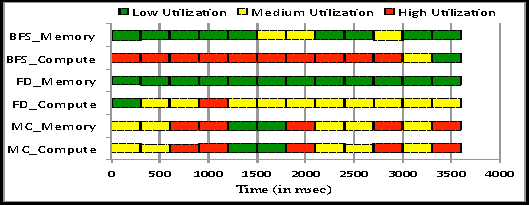
\includegraphics[width=3.2 in]{figures/cloud-workload.pdf}
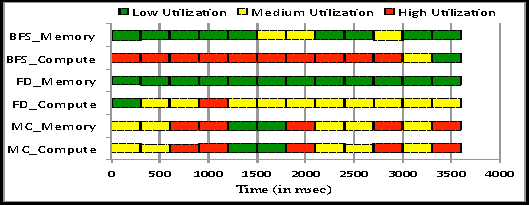
\includegraphics[width=0.75\textwidth,height=\textheight,keepaspectratio]{figures/cloud-workload.pdf}
\caption{Compute and memory characteristic of various GPU-based cloud applications. }
\label{fig:cloud-workload}
%\vspace{-1\baselineskip}
\end{figure}

\begin{figure}[t]
\centering
%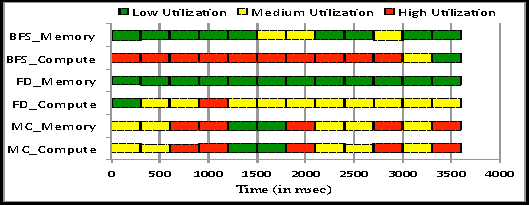
\includegraphics[width=3.2 in]{figures/cloud-workload.pdf}
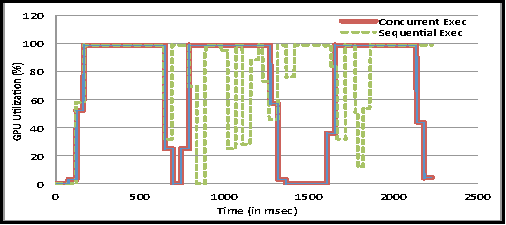
\includegraphics[width=0.75\textwidth,height=\textheight,keepaspectratio]{figures/GPU-utilization.pdf}
\caption{GPU utilization of Monte Carlo requests following exponential distribution of request arrival with sequential vs. concurrent execution. }
\label{fig:GPU-utilization}
%\vspace{-1\baselineskip}
\end{figure}

Another issue with current GPU programming models is that although each GPU can internally contain thousands of cores, application uses it as a single SIMD engine~\cite{GPU25}, which means that the multiple GPU contexts created by host threads can share a GPU only over time, but not in space. CUDA 4.0 addresses this problem by allowing multiple threads within a single host process to share the same GPU context, but GPU utilization could be improved further with true GPU multi-tenancy. We demonstrate this opportunity by manually dispatching multiple sets of independent Monte Carlo requests, again following an exponential distribution of inter-arrival times, over different CUDA \textit{Streams}~\cite{cuda7} from the same GPU context. Figure~\ref{fig:GPU-utilization} shows GPU usage peak and idle periods to be much more uniform compared to their sequential execution. This is because keeping a single GPU context avoids context switching overhead and this eliminates unnecessary GPU idling during context switching (the `glitches' in the figure), as in the case of independent sets of web requests driving their execution.

The illustrative examples above motivate key properties of the  Strings  approach  to effective multi-tenancy in GPU-based servers: (1)  load  balancing is needed to avoid static collisions, (2) device-level scheduling must be cognizant of character collisions   and   provide  such feedback  to  the   load  balancer,  (3)   additional   functionality   is  needed  to  achieve resource management goals like fairness, high throughput, etc., and (4) there should be system-level support for reducing GPU core idling when some application's context cannot fully utilize a single GPU. We next describe the Strings infrastructure and its utility for realizing and experimenting with effective scheduling strategies for cloud and multi-tenant workloads using GPUs.

\begin{figure}[!t]
\centering
%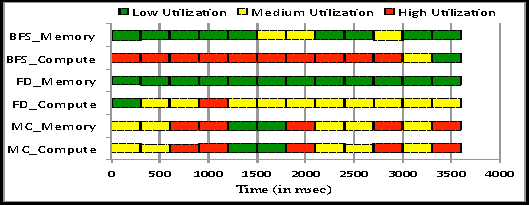
\includegraphics[width=3.2 in]{figures/cloud-workload.pdf}
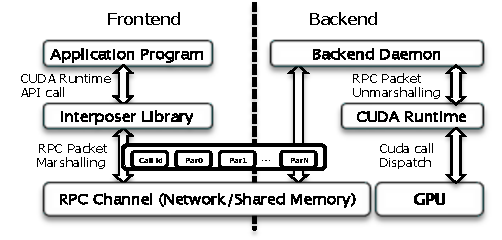
\includegraphics[width=0.85\textwidth,height=\textheight,keepaspectratio]{figures/GPU-remoting.pdf}
\caption{Architecture of GPU Remoting. }
\label{fig:GPU-remoting}
%\vspace{-1\baselineskip}
\end{figure}
\section{System Design Principles}
\subsection{Future GPU Servers and gPool}
Scheduling the potentially multiple GPUs in future server platforms demands (i) the logical aggregation of all GPUs to make them visible to the scheduler and then (ii) decoupling the CPU-GPU associations programmed into GPU-based applications. Strings adopts from previous work (e.g., GVim~\cite{gvim}, vCuda~\cite{vcuda}, rCuda~\cite{rcuda}, Pegasus~\cite{pegasus}, gVirtus~\cite{gvirtus}) an API-driven separation of an application's CPU from its GPU components. As shown in Figure~\ref{fig:GPU-remoting}, (i) a \textit{frontend} implemented as a CUDA runtime interposer library dynamically links with the application, responsible for intercepting the CUDA runtime API calls, and (ii) a \textit{backend} is realized as a daemon responsible for receiving GPU requests from the frontend, dispatching the CUDA runtime library calls to the attached GPUs, and returning error codes and/or output parameters to the frontend. A useful side effect of this architecture is the ability to execute an application's GPU component on a GPU attached to some remote node, termed GPU remoting~\cite{shadowfax}. We do not explore this topic at scale, but use it to create a supernode, which is an emulated high-end multi-GPU server machine   with  more  GPUs  than  those  available  on  today's single physical platforms. For such a supernode, Strings aggregates all GPUs into a single logical pool, termed a \textit{gPool}, for use by the GPU scheduler. The gPool is formed when the GPU virtualization runtime is started and the backend daemons are spawned in each participating node. Each backend collects the information of GPUs in its own node and sends it to the \textit{GPU Affinity Mapper}, discussed later. It assigns a unique GPU id (GID) to each of the GPUs in the pool, builds a mapping from GID to  \verb|<node_id (IP address), local device_id> |pair, called the \textit{gMap}, and broadcasts it to all participating machines.  

With  gPools,  gMap,  and  GPU  request  interposition,  the \textit{Strings} scheduling infrastructure described in this chapter permits any node in the gMap to participate in GPU scheduling. Figure~\ref{fig:GPool} shows the logical transformation of a small number of machines with per-node GPUs into a single supernode with sets of GPUs schedulable via a shared GPU pool. The experimental results in this chapter are obtained with a dual-machine supernode connected via dedicated network links. This purposely small scale setup makes it possible to treat remote GPUs much like NUMA memory is treated in high end servers, ignoring issues like network contention likely to occur for scaleout systems~\cite{shadowfax}.
\begin{figure}[!t]
\centering
%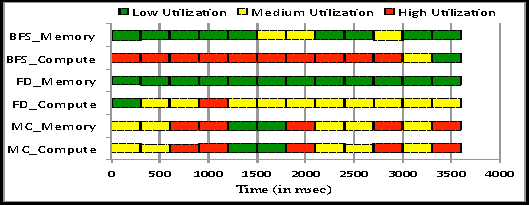
\includegraphics[width=3.2 in]{figures/cloud-workload.pdf}
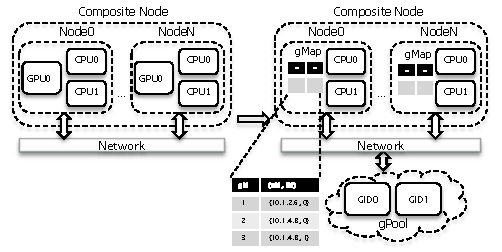
\includegraphics[width=\textwidth,height=\textheight,keepaspectratio]{figures/GPool.pdf}
\caption{Logical transformatiom of GPU cluster after gPool creation. }
\label{fig:GPool}
%\vspace{-1\baselineskip}
\end{figure}
\begin{figure}[!t]
\centering
%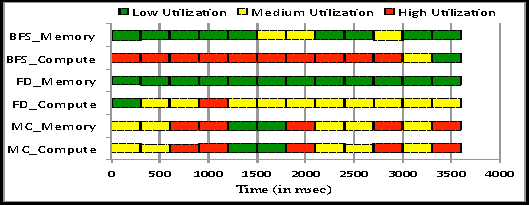
\includegraphics[width=3.2 in]{figures/cloud-workload.pdf}
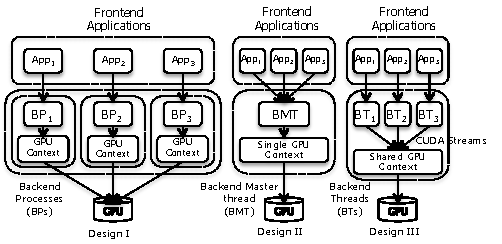
\includegraphics[width=\textwidth,height=\textheight,keepaspectratio]{figures/Strings-design.pdf}
\caption{Three different implementations GPU remoting.}
\label{fig:Strings-design}
%\vspace{-1\baselineskip}
\end{figure}

\subsection{Design Decisions}
\textbf{\textit{1) Efficient and Robust Scheduling}}

The frontend/backend model suggests three methods for mapping frontend applications to backend workers (processes or threads), shown in Figure~\ref{fig:Strings-design}.

\textbf{Design I.} 
Each frontend application is mapped to a unique backend process, which then dispatches the actual accelerator (e.g., CUDA) calls to some physical GPUs. This design offers high fault tolerance and security to frontend applications, as it isolates their GPU components in separate backend protection domains (GPU contexts). While used in our previous `Rain' scheduler~\cite{Rain}, as indicated in the figure, a drawback is that a large number of frontend applications will require an equally large number of backend processes, hurting scalability. For NVIDIA GPGPUs, because the CUDA runtime does not allow two different host processes to share the same GPU context, the GPU components of two different applications cannot run concurrently on a single GPU, resulting in GPU context switching overhead and potential GPU core idling.

\textbf{Design II.}
 An alternative design avoids context switching, by packing different application contexts into a single protection domain~\cite{liedtke}, which we term `context packing'. Specifically,   by   mapping   each   frontend   application  to  a different CUDA Stream~\cite{GPU5, ravi}, the design creates a single backend thread per device, thus consolidating the GPU components of all frontend applications into a single hosted GPU context. Advantages include (i) minimal backend context switching  overheads,  reduced  further by pinning the per GPU backend threads to certain CPU cores, and (ii) the presence of a single GPU context hosting all frontend applications, which enables the cross-application space-shared use of GPU resources – multi-tenancy. Such efficient GPU space sharing is useful for multi-tenant cloud workloads less concerned with isolation (e.g., Amazon's web store runs multiple web servers in a single VM, for efficiency in resource usage). It is also useful for pairing applications with different characteristics, e.g., one with high memory bandwidth, the other highly compute   intensive,   but  with  their  aggregate  GPU  resource requirements not exceeding those available in the physical GPU. An advantage specific to CUDA is (iii) that by leveraging CUDA streams, all three GPU engines, (a) memory copy from host to device (H2D), (b) from device to host (D2H), and (b) compute, can be concurrently used by different applications, to fully utilize these GPU resources. Potential shortcomings of the design are that (1) it is susceptible to faults, e.g., if the master thread managing all requests to a particular GPU crashes, all frontend applications relying on it are affected, (2) a malicious application can corrupt the entire GPU context or gain unauthorized access to other application’s data, (3) the single master thread has to continuously synchronize with all frontend applications to ensure fair overall progress and pipelined execution, which significantly adds to the complexity and overhead of the runtime, and (4) a blocking call, e.g., cudaDeviceSynchronize(), made by one application will block all other applications sharing the same GPU context, and deferring such call for a long time will lead to application starvation.

\textbf{Design III.} 
Strings adopts a hybrid of Designs I and II, leveraging the fact that for NVIDIA GPUs, from CUDA v4.0 onwards, GPU contexts are hosted per process per device, which implies that the GPU operations invoked from threads within a single host process can run concurrently on a GPU, while those from separate processes are still multiplexed by the device driver. As shown in Figure~\ref{fig:Strings-design}, in Strings, therefore, the GPU components of all frontend applications sharing a particular GPU are mapped to separate backend threads of the same per GPU backend process, with their respective GPU operations invoked via separate CUDA streams. The design has reduced overhead compared to Design I, due to reduced thread vs. process context switch overheads. While not providing complete isolation, the design improves on Design II in that faults can be localized to certain threads. Most importantly, the GPU operations from different applications can run concurrently, thereby inheriting all of the benefits of space and time sharing of Design II. Further, as GPU requests are channelized through separate backend threads, overheads of request synchronization and of pipelined execution are reduced to a minimum, and properties like fair progress for GPU applications are much easier to implement.

\textbf{\textit{2) Asynchronous Operation}}

The presence of an explicit interposer affords additional optimizations. First is the removal of blocking calls, by converting all device synchronization calls to their respective stream synchronization counterparts, e.g., cudaDeviceSynchronize() converted to cudaStreamSynchronize(). This ensures that all the applications sharing a GPU, under the umbrella of a single GPU context, are not stalled when one application explicitly synchronizes with the device.

Second is the runtime conversion of all synchronous memcpy operations into their respective asynchronous versions. With this optimization, (i) subsequent CUDA calls that are not dependent on the memcpy operation can proceed without waiting for memcpy calls to finish, (ii) we hide the overhead introduced by the runtime due to interposition, marshaling, RPC, unmarshalling etc, by allowing execution to proceed and overlap even for calls that are dependent on the memcpy operation. For instance, a cudaLaunch() call that depends on a memcpy typically has to wait for the memcpy to complete, but because it is now asynchronous, the runtime layer overhead for cudaLaunch() can be overlapped with the asynchronous data transfer to the device.

Finally, asynchrony can also be achieved for hidden and synchronous runtime API calls that do not have output parameters, by making interposer-based RPCs non-blocking. This does not violate the correctness in single threaded applications as RPC requests from within an application remain in-order but might affect multi-threaded applications where RPCs from separate threads are not guaranteed to be in-order e.g., when cudaLaunch() from one host thread depends on a memcpy from another and an asynchronous RPC makes the former call to be dispatched before the latter. The problem can be corrected with per-device buffer synchronization logic that maintains the application-intended order of GPU operations across multiple threads within a single application.
\begin{figure}[!t]
\centering
%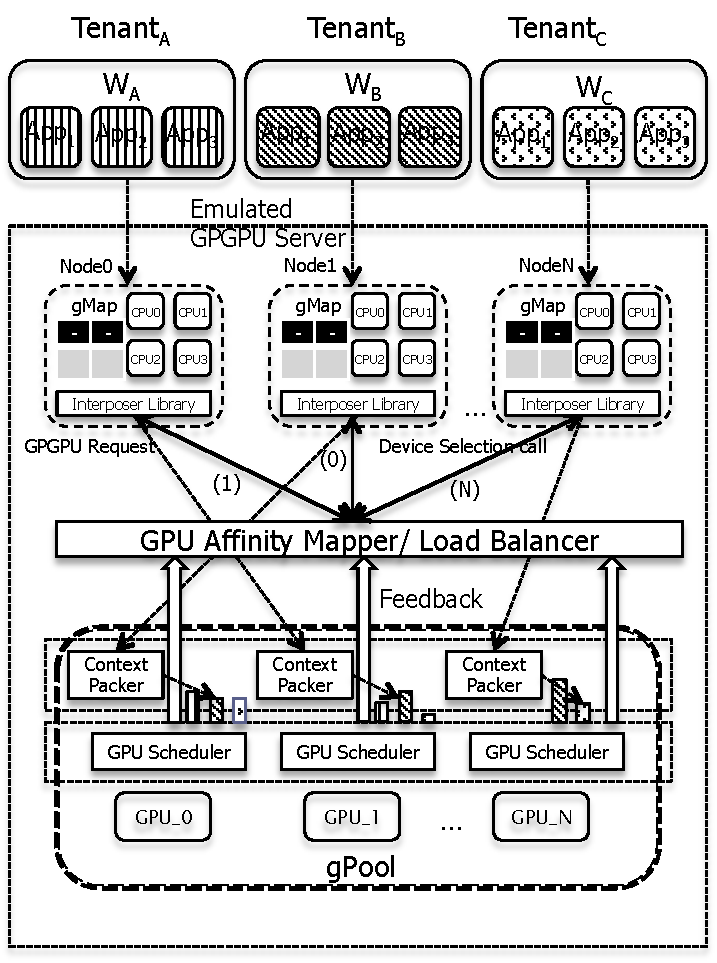
\includegraphics[width=\textwidth,height=\textheight,keepaspectratio]{figures/strings_archi1.pdf}
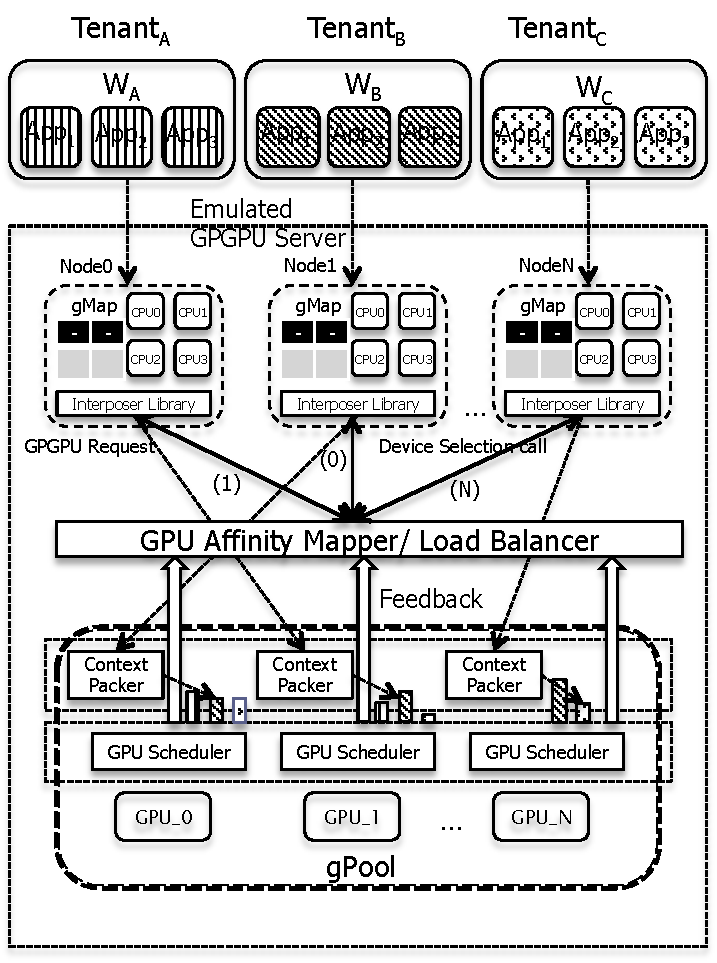
\includegraphics{figures/strings_archi1.pdf}
\caption{Software architecture of Strings.}
\label{fig:strings_archi}
%\vspace{-1\baselineskip}
\end{figure}
\section{Strings Architecture}
We next describe the two-level Strings scheduling infrastructure that avoids static and character collisions of GPU requests, efficiently utilizes the underlying GPU cores with minimum GPU context switching overhead, and meets system goals like throughput and fairness (see Figure~\ref{fig:strings_archi}).

\textbf{GPU Affinity Mapper - Workload Balancing. }To minimize static collisions, the Strings runtime overrides the application's target GPU selection calls, replacing them with decisions made by the GPU affinity mapper/workload balancer. The lifetime of the Strings target device selection call is as follows: (i) an application's cudaSetDevice() call is intercepted by the interposer and forwarded to the workload balancer; (ii) its GPU selection based on static (device capabilities) and dynamic (GPU load, application type, feedback from lower scheduling layer) parameters is returned as a global GPU id (GID) to the interposer; (iii) the interposer uses the GID to acquire a node id and local GPU id from the gMap, and (iv) using GPU remoting, it then forwards the call to some appropriate backend process to bind with the target GPU; (v) the binding is removed when the application exits or calls cudaThreadExit(). The \textit{GPU Affinity Mapper} is also responsible for the cluster-wide aggregation of GPUs through gPool creation. Shown in Figure~\ref{fig:affinity}, it has the following components:
\begin{figure}[!t]
\centering
%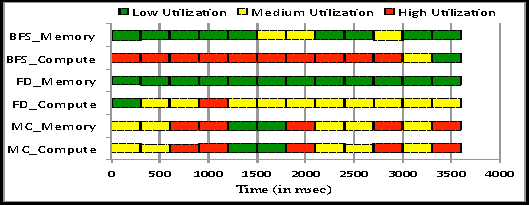
\includegraphics[width=3.2 in]{figures/cloud-workload.pdf}
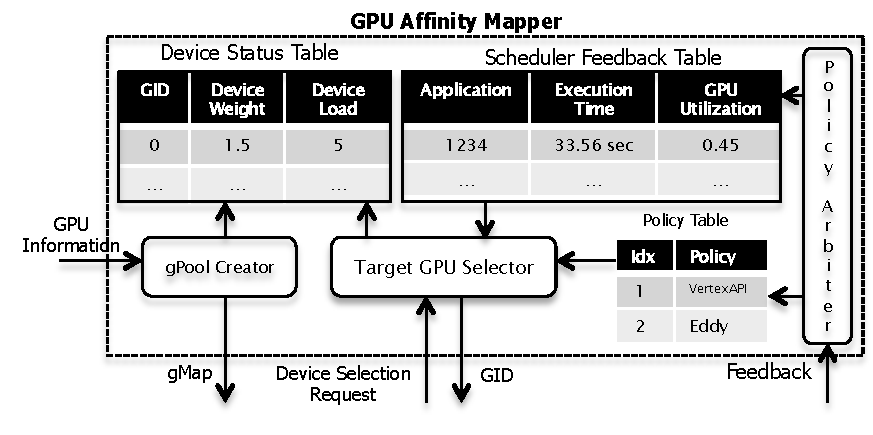
\includegraphics[width=\textwidth,height=\textheight,keepaspectratio]{figures/strings_archi2.pdf}
\caption{The structure of the GPU Affinity Mapper.}
\label{fig:affinity}
%\vspace{-1\baselineskip}
\end{figure}
\begin{itemize}
\item \textbf{\textit{gPool Creator (GC): }}during system initialization, the GC collects device information from the backend daemons of each  node  in  the cluster, assigns a GID to every GPU, creates the gMap and broadcasts it to every node. GC is also responsible for the one time assignment of relative weights to all GPUs based on the device property information received and updating a global data structure, Device Status Table (DST), with this static information. DST also maintains the dynamic states (e.g. current device load) of all the GPUs in the system, which is updated by TGS (explained later) as GPU requests arrive. 
\item \textbf{\textit{Policy Arbiter (PA): }}using the feedback mechanism, the PA receives information about application characteristics like execution time, GPU utilization, data transfer time etc. from the Feedback Engine (FE) of the device-level GPU schedulers and updates a history-based table, Scheduler Feedback Table (SFT), that stores such fine-grain device specific application characteristic information. The PA also triggers dynamic policy switching, upon receiving sufficient feedback information from low-level GPU schedulers.
\item \textbf{\textit{Target GPU Selector (TGS): }}as the core of the workload balancer, it selects an appropriate GPU for an application. Based on the information in the DST and SFT, for each GPU selection request, it computes the target GID using the selected scheduling policy from the Policy Table (PT) and then returns it to interposer, which then maps the application to a particular GPU in gPool. The PT contains two classes of policies, one that uses only the DST, e.g., GRR, GMin, etc., and the other that uses both the DST and low-level feedback information from SFT, e.g., GUF, DTF, etc.
\end{itemize}
\begin{figure}[!t]
\centering
%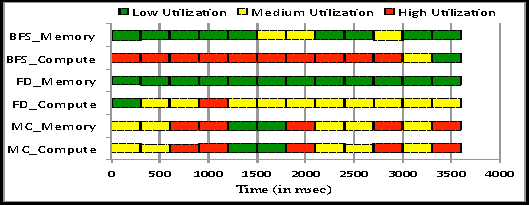
\includegraphics[width=3.2 in]{figures/cloud-workload.pdf}
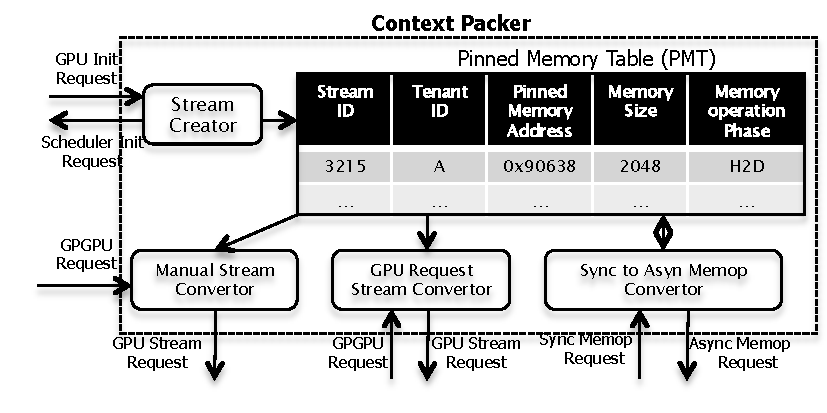
\includegraphics[width=\textwidth,height=\textheight,keepaspectratio]{figures/strings_archi3.pdf}
\caption{The structure of the Context Packer.}
\label{fig:packer}
%\vspace{-1\baselineskip}
\end{figure}
\textbf{Context Packer. } Operating after workload load balancing has assigned a GPU and before device-level GPU scheduling, the Context Packer (see Figure~\ref{fig:packer}), is responsible for packing multiple applications' GPU components that share a GPU, on the fly, into a single GPU context. It also manages the host side locked memory, the dynamic translation of synchronous memory copies to their asynchronous versions, and the dynamic translation of device synchronization calls to their stream counterparts.
\begin{itemize}
\item \textbf{\textit{Stream Creator (SC): }}when the first GPU request from an application arrives, SC creates a separate CUDA stream object for it, calling cudaStreamCreate(), the handler to which is stored in a thread local storage. Using this handler, subsequent requests from the application are dispatched over the stream. On cudaThreadExit() or application exit, SC tears down the stream by calling cudaStreamDestroy() on the stream handler.
\item \textbf{\textit{Auto Stream Translator (AST): }}dynamically translates all GPU operations from an application targeted over the default  stream  (stream 0)  to use the stream created by the SC. E.g., cudaConfigureCall(),   when  called  without  an  explicit stream handler in its call parameters, is targeted onto stream 0, and  AST uses the stream handler for this particular application to translate the call to use that stream.
\item \textbf{\textit{Sync Stream Translator (SST): }}the GPU calls that synchronize the application and the device are converted to their CUDA stream counterparts by the SST, e.g., cudaDeviceSynchronize()    is     converted    to     cudaStreamSynchronize(). This ensures that all of the applications packed into a GPU context associated with a particular GPU are not blocked when one of them explicitly tries to synchronize its host thread with the device. 
\item \textbf{\textit{Memory Operation Translator (MOT): }}translates all memory copies to their asynchronous versions using a per device data structure called Pinned Memory Table (PMT).  PMT stores the active host and device pointers associated with all such memory copy calls and is also responsible for keeping track of the current memory copy phase (e.g., H2D) of an application, storing the stream handler, the application id, tenant id, etc. MOT allocates host locked memory of the size of the host buffer for every such memory copy operation, copies the content of the host buffer into it, and stores both the host and device pointers in the PMT. It then creates an asynchronous version of the memory copy call (e.g. cudaMemcpyAsync()) using the host pointer. On the application’s next device synchronization call or a device to host memory copy, the MOT searches for the device pointer in the PMT and frees the corresponding host memory. When the application invokes the cudaThreadExit() or exits, the MOT frees all outstanding active host pointers in the PMT associated with the application.
\end{itemize}
\begin{figure}[!t]
\centering
%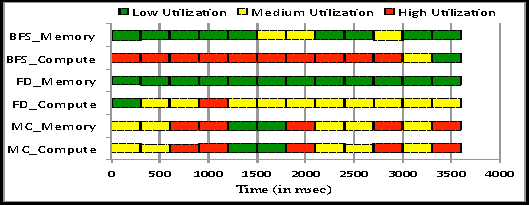
\includegraphics[width=3.2 in]{figures/cloud-workload.pdf}
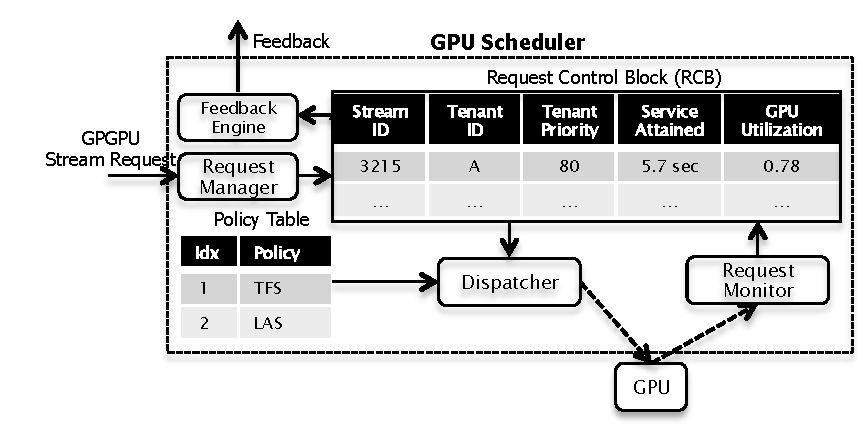
\includegraphics[width=\textwidth,height=\textheight,keepaspectratio]{figures/strings_archi4.pdf}
\caption{The structure of the GPU Scheduler.}
\label{fig:sched}
%\vspace{-1\baselineskip}
\end{figure}
\textbf{GPU Scheduler. }As shown in Figure~\ref{fig:sched}, this per device software layer addresses inter-application interference arising due to the co-location of multiple applications' GPU components on a single GPU. It prioritizes and dispatches GPU requests to physical GPUs in order to meet resource management goals like system throughput, fairness, etc. It is also responsible for monitoring applications bound to the device and sending feedback about their characteristics to the workload balancer.
\begin{itemize}
\item \textbf{\textit{Request Manager (RM): }} registers and unregisters application requests with the GPU scheduler. After the GPU affinity mapper selects the target GPU for an application, the interposer library makes a cudaSetDevice() call to the selected GPU using the GPU remoting infrastructure. On receiving the request, the RM registers the application by creating an entry in a per device data structure called Request Control Block (RCB) with stream id, tenant id and application priority, to be used by the GPU scheduler. RCB also maintains application runtime characteristic information, dynamically computed by the Request Monitor discussed later. When the interposer forwards a cudaThreadExit() call, the RM unregisters the application by removing its corresponding entry from the RCB.
\item \textbf{\textit{Dispatcher: }}prioritizes and dispatches GPGPU requests to the device. It uses the application characteristic information from the RCB and makes scheduling decisions based on the selected policy from the Policy Table (PT). In Strings three policies are implemented to achieve system fairness (TFS), high system throughput (LAS), and a combination of fairness and system throughput (PS).
\item \textbf{\textit{Request Monitor (RMO): }}computes GPGPU application characteristics and GPU resource usage. Both the workload balancer and GPU scheduler make use of this monitoring information in their scheduling decisions. We currently monitor the total execution time, total GPU time, data transfer time, memory bandwidth, application phase and kernel configuration information of an application. The RMO updates RCB in some regular time interval.
\item \textbf{\textit{Feedback Engine (FE): }}communicates the application characteristic and local GPU state information, collected by the RMO, to the GPU Affinity Mapper. It retrieves this information from the RCB and feeds it to the SFT when the application request completes. Therefore, when a cudaThreadExit() call arrives, FE piggybacks the feedback information along with the return value of the CUDA call and sends it back to the interposer, which then forwards the same to the GPU Affinity Mapper.
\end{itemize}

\section{Scheduling Policies}
Strings  implements  a  rich  set  of  scheduling  policies,  to achieve two cloud- and server-centric goals: fairness for multiple tenants, coupled with high overall system throughput.
\subsection{Workload Balancing Policies }
Three workload balancing policies across multiple accelerators are suitable for server systems, driven by external workloads like those seen for cloud and web applications.
\begin{itemize}
\item \textbf{\textit{Global Round Robin (GRR): }}assigns incoming applications to the GPUs in the gPool in a round robin fashion.
\item \textbf{\textit{GMin: }} taking into account the differences in application runtimes, GMin enhances GRR by maintaining a record of the number of applications currently bound to a particular device in the \textit{device load} field. GMin chooses the GPU with minimum device load. Because remote GPUs are more expensive to access, GMin breaks ties by giving preference to local GPUs over remote ones.
\item \textbf{\textit{Weighted-GMin: }}considering heterogeneity across GPUs, in terms of compute, memory capacity and bandwidth, the weighted-GMin (GWtMin) policy extends GMin by assigning relative weights to different GPUs and computing weighted minimum load to select a target GPU.
\end{itemize}
\begin{figure}[!t]
\centering
%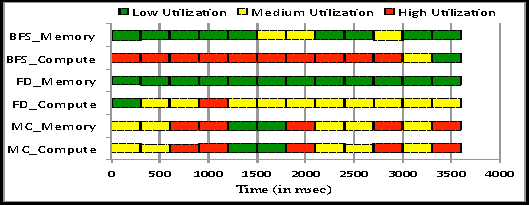
\includegraphics[width=3.2 in]{figures/cloud-workload.pdf}
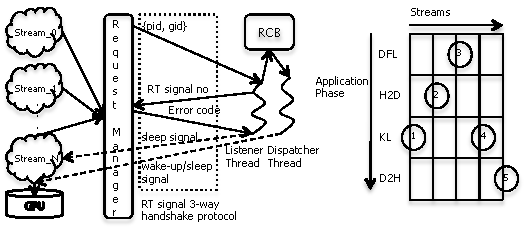
\includegraphics[width=\textwidth,height=\textheight,keepaspectratio]{figures/RT_sched.pdf}
\caption{(a) Real-Time Signal based GPU Scheduler (b) Phase Selection Scheduling Policy. }
\label{fig:RT_sched}
%\vspace{-1\baselineskip}
\end{figure}
\subsection{GPU Scheduling Policies}
Once workload balancing has been done, GPU scheduling policies concern fairness- and system throughput.
\begin{itemize}
\item \textbf{\textit{Least Attained Service (LAS): }} a GPU-based application, after offloading work to the GPU, uses the CPU until it issues a call, e.g., cudaDeviceSynchronise(), that requires it to wait for the completion of previously issued GPU work. The objective of LAS is to minimize this CPU `stall time' and thereby maximize system throughput, by prioritizing jobs with least attained service time~\cite{queue}. The policy works by increasing the priority levels of those applications that have attained less GPU service time in a given time quantum. This enables the applications with shorter GPU episodes to finish sooner, thereby reducing overall CPU stall time and improving system throughput. The time quantum chosen in LAS is larger than the time slice assigned to each backend thread by the GPU scheduler, to ensure that an application's GPU characteristic is determined for its long-term behavior. LAS also uses a time decaying GPU service time formula~\cite{atlas}, to give higher weight to more recent service epochs.
\begin{equation}
             CGS_n = k*GS_n + (1-k)*CGS_{n-1} 
\end{equation}
$CGS_n$: \textit{Cumulative GPU service time attained till $n^{th}$ epoch}

$GS_n$ : \textit{GPU service time attained in the nth epoch and k = 0.8.}

\hfill \break
The next set of GPU scheduling policies are implemented using Unix Real-time (RT) signals. Figure~\ref{fig:RT_sched}a shows the three-way handshake protocol followed during the application registration phase: (1) the backend thread corresponding to the GPU application registers its stream id, tenant id, and tenant weight with the RM using IPC; (2) the listener thread of the RM, on receiving the request, creates an entry in the RCB, sends the next available RT signal id to the backend thread; (3) the backend thread, on receiving it, installs a signal handler and sends the error code as an acknowledgement to the RM. The signal handler registered ensures that the backend thread toggles between its sleep and wake-up states on receiving its assigned RT signal. The Dispatcher, which is responsible for prioritization of GPU requests, uses this mechanism to control which backend threads should be using the GPU and for how long. 

\item \textbf{\textit{True Fair-Share (TFS): }}to ensure fairness among multiple tenants sharing the same GPU, the TFS scheduler ensures a proportionate GPU resource allocation on a per-tenant basis according to their assigned weights. The Dispatcher realizes this by keeping registered backend threads awake only for a time period that is proportional to their tenant weights.  The invariant maintained by the Dispatcher is that at any point of time, at most one backend thread is awake and is using the GPU. To  address  unfairness  in  GPU  access  across applications with long vs. short GPU episodes, TFS maintains a history of GPU usage over the past scheduling epochs, and if any application overshoots its allocated time slice, the dispatcher penalizes it in subsequent epochs. Thus, TFS ensures that tenants receive their weighted fair share under high system load and its work-conserving nature distributes a tenant’s unused shares among the applications of other tenants according to their respective weights.

\item \textbf{\textit{Phase selection (PS): }}CUDA streams can leverage the parallelism opportunities offered by multiple hardware queues (data transfer and compute) present in NVIDIA GPUs. Specifically, if the GPU scheduler receives a cudaLaunch(), cudaMemcpy() Host to Device (H2D) and Device to Host  (D2H) at around the same time from three different backend threads, all of them can be serviced concurrently, as the calls are sent over different streams belonging to the same GPU context. To take advantage of this, the backend threads keep the GPU scheduler apprised of their current GPU usage phase, the Dispatcher identifies threads that are in different GPU phases, and wakes them up. If it cannot find at least one thread from each of the GPU phases, it wakes up threads in the following priority order: Kernel Launch $(KL) > H2D = D2H > $ Default Phase (DFL). Note that this policy relaxes the TFS invariant of keeping only one backend thread awake in any scheduling epoch. The dispatcher picking threads in different phases of their execution has some similarity with playing a guitar chord (Figure~\ref{fig:RT_sched}b), by pressing a set of strings at specific frets. Our GPU scheduling framework derives its name `Strings' from this analogy.
\end{itemize}

\subsection{Feedback-based Load Balancing}
It is important to assess accelerator utilization when scheduling   its   resources,   particularly  for  applications  with dynamic usage profiles. Feedback-based policies use such device-level information to guide load balancing.
\begin{itemize}
\item \textbf{\textit{Runtime Feedback (RTF): }} the GPU Scheduler monitors the execution time of requests scheduled on the GPU and provides such feedback to the workload balancer, which uses this to improve future GPU assignments. 
\item \textbf{\textit{GPU Utilization Feedback (GUF): }}the   GPU  Scheduler provides  feedback  to  the workload balancer about how efficiently an application is using the GPU, by computing GPU utilization, as the ratio of the total GPU time of an application to its total runtime. Borrowing from NUMA-aware  thread placement~\cite{numa}, GUF tries to avoid collocation of applications with  high  GPU  utilization  on  the  same  GPU. Decisions are refined over time as the system learns about the GPU characteristics of more applications from the feedback mechanism.
\item \textbf{\textit{Data Transfer Feedback (DTF): }}DTF capitalizes on CUDA streams to overlap device-level computation with data transfers between host and device. By providing feedback to the workload balancer about the time spent on data transfer, it becomes possible to collocate applications with differing characteristics, some being transfer- and others being compute-intensive.
\item \textbf{\textit{ Memory Bandwidth Feedback (MBF): }}the MBF policy uses as input from device-level scheduling the approximate memory bandwidth of an application, by taking the ratio of the total data accesses by its computation kernels to the total time spent on the GPU. Workload balancing uses this information to avoid collocating   bandwidth-bound   threads.   Resulting   performance improvements leverage the fact that GPU-resident non-bandwidth/compute bound threads can hide the memory latencies experienced by bandwidth-bound GPU kernels.
\end{itemize}
\subsection{Discussion}
Important and novel about the GPU scheduling policies described above (vs. those targeting CPUs) is the explicit attention paid to data movement to/from GPUs. Phase Selection (PS) attempts to schedule requests differing in the phases in which they operate: computing vs. moving data. Feedback not only concerns GPU execution, but also to distinguish compute- from more movement-intensive GPU requests, refined by one specific quantification of memory movement: the approximate level of memory bandwidth consumed by GPU requests. While the implementation of these functionalities in the current Strings system is for CUDA devices, they are equally important for other accelerators, including those integrated into the platform (e.g., AMD’s Fusion architecture) and those using alternative accelerator architectures (e.g., Intel’s Xeon Phi).

\begin{table*}[!t] 
%\caption{{BENCHMARK APPLICATIONS}}
\caption{{Benchmark Applications}}
\centering 
%\vspace{-0.2cm}
\label{tbl:table} 
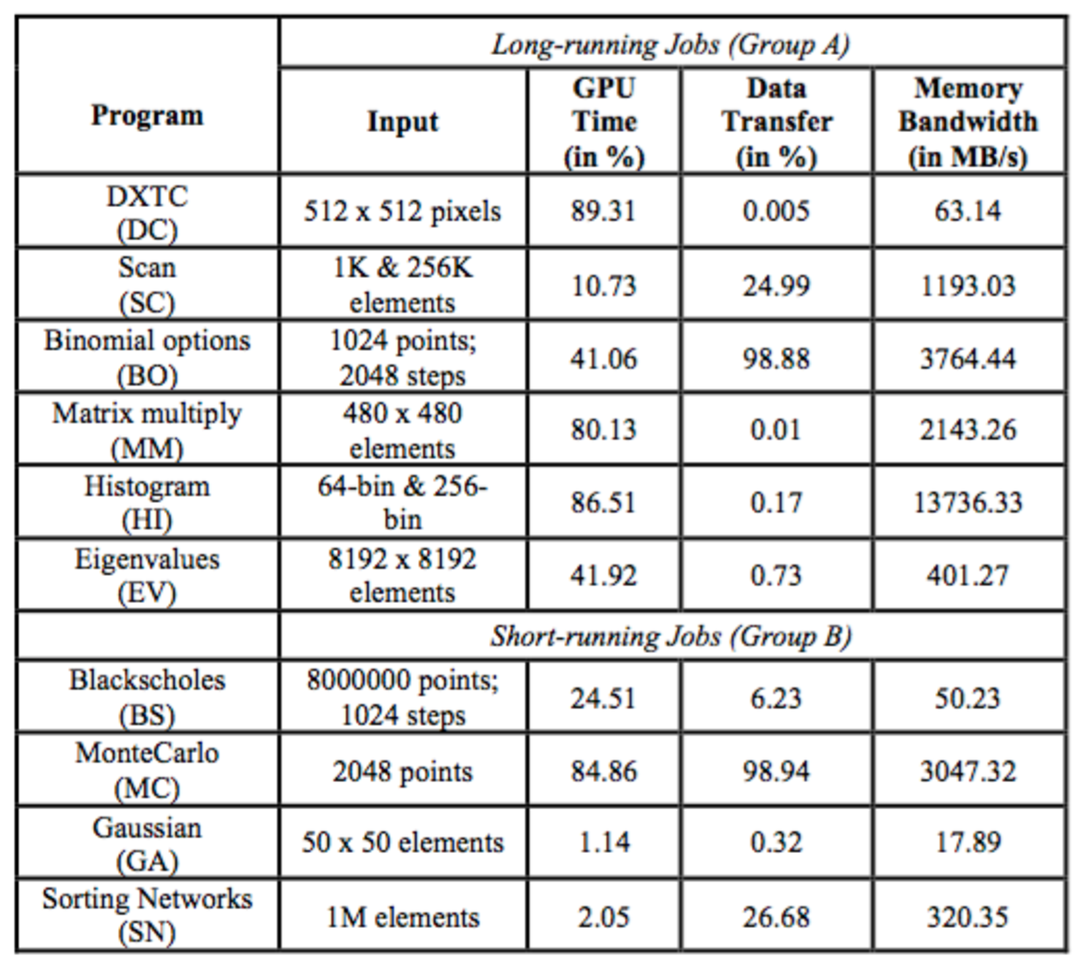
\includegraphics[width=0.9\textwidth,height=\textheight,keepaspectratio]{figures/Strings_Table.pdf}
%\vspace{-0.5cm} 
\end{table*}

\begin{figure}[t]
\centering
%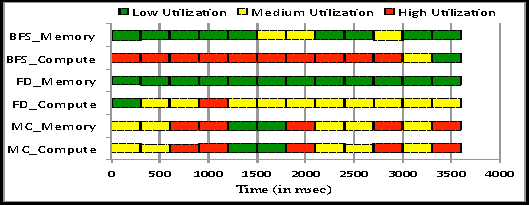
\includegraphics[width=3.2 in]{figures/cloud-workload.pdf}
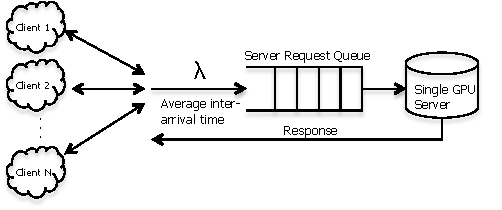
\includegraphics[width=0.80\textwidth,height=\textheight,keepaspectratio]{figures/servicemodel.pdf}
\caption{GPGPU application service model following a negative exponential distribution of request arrival from multiple end users.}
\label{fig:servicemodel}
%\vspace{-1\baselineskip}
\end{figure}
\section{Experimental Evaluation}
The purpose of the experimental evaluations shown below is twofold. First, they show the importance of explicit accelerator scheduling for the cloud and server workloads seen in future datacenter systems. Second, device-level feedback about application characteristics and behavior is shown to be critical for obtaining high throughput and efficiently utilizing accelerator resources.
\subsection{Evaluation Metrics}
We use weighted speedup~\cite{dean} and Jain's fairness~\cite{jain} as metrics to measure overall system throughput and fairness, respectively. Weighted speedup measures the average speedup in an application when running alone compared to when the application  is sharing the GPU. The  fairness  metric  measures per-application fairness achieved when two or more applications share the GPU where each is allocated a pre-defined share of the resource.
\begin{equation}
Weighted\  Speedup = \frac{1}{N}*\sum_{i=1}^{N}\frac{T_i^{alone}}{T_i^{shared}} 
\end{equation}

\begin{equation}
Jain's\ Fairness = \frac{(\sum_{i=1}^N\frac{T_i}{W_i})^2}{N*\sum_{i=1}^N(\frac{T_i}{W_i})^2}
\end{equation}
\subsection{Benchmarks}
Applications from the CUDA SDK and the Rodinia benchmark suite~\cite{rodinia}, listed in Table~\ref{tbl:table}, are chosen to create a pairwise workload mix of short ($<$ 10sec) and relatively long (10-55 sec) running jobs. 24 such workload pairs are used, labeled from A to X, where A is the DC-BS pair, B is the DC-MC pair, X is the EV-SN pair, and so on, following the order in Table~\ref{tbl:table}. We assume typical cloud services to operate in response to end user requests, with each individual service running for some small amount of time to complete a single request, but with the requirement of being highly responsive. This assumption matches the service behavior reported by Amazon, for instance, for its web service infrastructure. However, the actual types of service instances being used will vary, which we reflect by carefully choosing for the evaluation a diverse set of application kernels, like image processing (e.g., matrixmult), financial (e.g., BlackScholes), etc. The outcome is a workload mix with many short running rather than a few long running sets of jobs.

\subsection{Experimental Setup}
Experiments are performed on two different classes of servers, a small-scale (two GPUs) server and a higher end (four GPUs) server emulated by a supernode comprised of two dedicated dual-GPU nodes (NodeA and NodeB) connected via Gigabit Ethernet. Each of the two machines is equipped with two Intel Xeon X5660 processors running at 2.8 GHz, for a total of 12 cores and 12 GB of RAM, and has two attached NVIDIA FERMI GPUs. NodeA has a Quadro 2000 and Tesla C2050, while NodeB has Quadro 4000 and Tesla C2070 GPUs, resulting in a supernode with a heterogeneous GPU pool where GPUs differ in terms of their compute and memory bandwidth capacities. The CUDA runtime and driver versions are 5.0 and 319.49, respectively. Our GPGPU application service model, as shown in Figure~\ref{fig:servicemodel}, is based on the SPECpower\_ssj2008 benchmark~\cite{spec}, which models a server application with a large number of end users. User requests follow a negative exponential distribution and are served by a finite  number  of  server  threads. The  exponential distribution models intermittent periods of bursts of load when application requests queue up while  other  requests are being processed, followed by  periods of  calm  when  the  accumulated  requests  are  serviced.  For a particular random stream of requests, the inter-arrival time between any two consecutive requests, can be calculated using the following formula:  
\begin{equation}
T = - \lambda*log(X)
\end{equation}
where $\lambda$ is the mean inter-arrival time between consecutive requests, and $X$ is a random number in the range (0.0, 1.0].

NodeA and NodeB are servers processing GPU application requests. In our small-scale server experiments, NodeA sees a stream of requests following a negative exponential distribution, as described above, with λ proportional to the application’s runtime. In the emulated high-end server experiments, each node sees independent random streams of requests. In both the small and large-scale server experiments the assumption is λ is large enough to handle the memory pressure on GPUs being shared, in other words GPU requests never pile up to the degree that they run out of device memory.
\begin{figure}[t]
\centering
%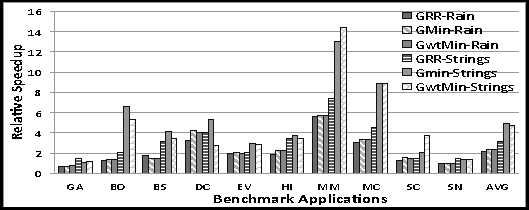
\includegraphics[width=3.2 in]{figures/strings_exp1.pdf}
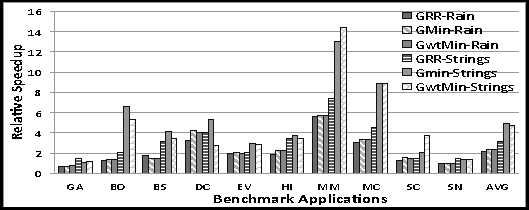
\includegraphics[width=0.75\textwidth,height=\textheight,keepaspectratio]{figures/strings_exp1.pdf}
\caption{Performance benefit of workload balancing policies vs. CUDA runtime in a single node with 2 GPUs.}
\label{fig:strings_exp1}
%\vspace{-1\baselineskip}
\end{figure}


\subsection{Results}
\textbf{Importance of Workload Balancing. }In this set of experiments with a small-scale server, a node receives a stream of requests for a particular application following a negative exponential distribution. As shown in Figure~\ref{fig:strings_exp1}, the average completion time of all requests served is calculated and compared with the different workload balancing policies of Rain and Strings with the baseline being CUDA runtime (relative speedup). We can observe that there is significant throughput improvement with both our former solutions, Rain, and also with Strings, because unlike the CUDA runtime, which respects the application’s target GPU selection, the workload balancer ignores it and dynamically distributes GPU requests across all GPUs in a node. This keeps both of the GPUs in the node busy, avoiding static GPU request collisions, thereby increasing the overall GPU utilization and achieving high system throughput. We also observe that every Strings workload balancing policy performs better than its Rain counterpart. This is because applications mapped to any GPU by Strings belong to the same GPU context and are dispatched over independent CUDA streams. This promotes concurrent execution (1) via time and space sharing the GPU and (2) by keeping both compute and memory copy engines of the GPU busy simultaneously. Averaged over all benchmark applications, the GRR-Rain, GMin-Rain, GWtMin-Rain, GRR-Strings, GMin-Strings and GWtMin-Srings policies achieve weighted speedups of 2.16x, 2.37x, 2.34x, 3.10x, 4.90x, and 4.73x,  respectively,  compared  to the CUDA runtime. Further, on average, Strings workload balancing performs up to 2.10x better than Rain. Interestingly, for some applications (BO, BS and DC), note that GMin outperforms GWtMin, although the latter is, in principle, a better scheduling policy. This is because the static GPU weights assigned to each GPU during system initialization, in many cases, do not mirror the actual relative differences in application performance and therefore, fail to account for diverse application characteristics. This is a  key motivation for feedback-based  load  balancing  evaluated later. In   Strings, for   the   workloads   Gaussian   and  Scan,  GRR performs better than GMin, which seems counter-intuitive. This happens because unlike Rain, in Strings, the per-GPU request queue length (used in the logic of the GMin policy) does not exactly capture the current load in the device. In Rain, the product of queue length and average application runtime in the queue is the total time for servicing the entire queue, but this is not true in Strings, with its multiple GPU requests serviced concurrently. 
\begin{figure}[h]
\centering
%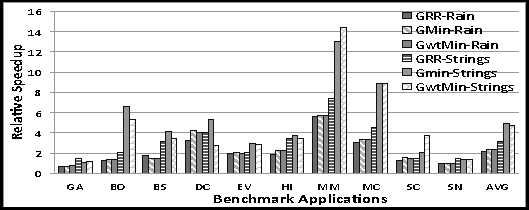
\includegraphics[width=3.2 in]{figures/strings_exp1.pdf}
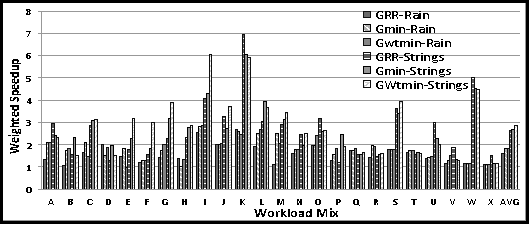
\includegraphics[width=0.75\textwidth,height=\textheight,keepaspectratio]{figures/strings_exp2.pdf}
\caption{Performance benefit of GPU sharing in an emulated 4 GPU server. }
\label{fig:strings_exp2}
%\vspace{-1\baselineskip}
\end{figure}
\begin{figure}[h]
\centering
%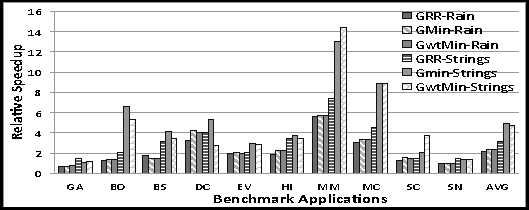
\includegraphics[width=3.2 in]{figures/strings_exp1.pdf}
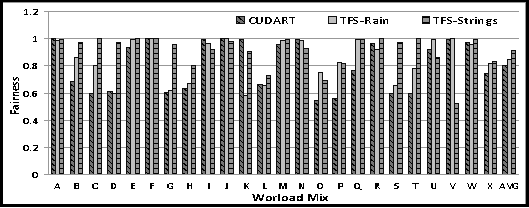
\includegraphics[width=0.75\textwidth,height=\textheight,keepaspectratio]{figures/strings_exp3.pdf}
\caption{Fairness achieved by TFS-Strings vs. TFS-Rain vs. CUDA runtime. }
\label{fig:strings_exp3}
%\vspace{-1\baselineskip}
\end{figure}

\textbf{Benefits of GPU Sharing.} Experiments with the emulated (two node) larger-scale server machine show the benefits of sharing GPUs among multiple application streams. In these experiments, one node receives a stream of longer running GPU requests (Group A) whereas the other receives a stream of shorter requests (Group B), for two different applications and following a negative exponential distribution. Leveraging the gPool, for these sets of requests, the workload balancer dynamically distributes them across all four GPUs in the supernode. Experiments record the average completion time of each application for each of the different workload balancing policies, with the baseline being the single node GRR policy. This means that the performance benefits reported are over and above those obtained with the single node GRR policy described in the previous section. As shown in Figure~\ref{fig:strings_exp2}, averaged over 24 workload pairs, taking one each from Group A and B, the speedups achieved by GRR-Rain, GMin-Rain, GWtMin-Rain, GRR-Strings, GMin-Strings, and GWtMin-Strings policies are 1.60x, 1.80x, 1.82x, 2.64x, 2.69x and 2.88x respectively. These speedups include the effects of both GPU sharing and workload balancing. These notable speedups are derived in part from the fact that the peaks in GPU requests from the two statistically independent streams are not aligned, thus allowing the workload balancer to distribute GPU requests efficiently among all four GPUs. We also observe that for all of the application pairs, maximum speedups are achieved in workloads (I, K and W) in which one of the applications is either BlackScholes or Gaussian. This is because for both of these benchmarks, relative GPU usage is among the lowest,  thus benefiting the other application in the workload mix. Namely, BlackScholes has the least total execution time while the Gaussian kernel has very low GPU utilization, minimal data transfer, and negligible memory bandwidth. Finally, Strings outperforms Rain in GPU sharing because (i) the effect of GPU sharing becomes even more prominent with the opportunity of concurrent execution of GPU requests, and (ii) as shown in the motivation section, a consolidated single GPU context per device makes GPU usage much more uniform, allowing the efficient collocation of multiple requests.

\textbf{Benefits of GPU Scheduling. }We next evaluate a fairshare (TFS) and two throughput-oriented (LAS and PS) GPU scheduling policies.

\textit{1) Fairshare  Scheduler: } in  this  set  of single node experi- ments,  application  pairs  share  a  single  GPU,  each  assigned equal GPU shares. From Figure~\ref{fig:strings_exp3}, we see that TFS-Strings outperforms both the CUDA runtime and the TFS-Rain scheduling policy. The average fairness achieved by TFS- Strings is 91\%, which is 13\% and 7.14\% better than the CUDA runtime and TFS-Rain, respectively. The maximum fairness achieved by TFS-Strings is close to ideal  (99.99\%), for the following reasons. By keeping a history of the GPU time attained by individual applications and penalizing any application in subsequent epochs that used the GPU for more than its allocated share in a previous epoch, both TFS-Rain and TFS-Strings  achieve  better  fairness  compared  to  the CUDA runtime. TFS-Strings achieving higher fairness compared to TFS-Rain might seem counter-intuitive, because the concurrently executing GPU requests from different applications in  Strings  makes  it  difficult  to  track or control fairness in GPU allocation. Better fairness in TFS-Strings can be explained by the fact that because there is no GPU context-switching among applications sharing a GPU in Strings, the error in the calculation of GPU usage of an application in a particular epoch is substantially reduced compared to that of Rain where the GPU context-switching overhead is included in the fairness calculation along with the application’s actual GPU usage.
\begin{figure}[t]
\centering
%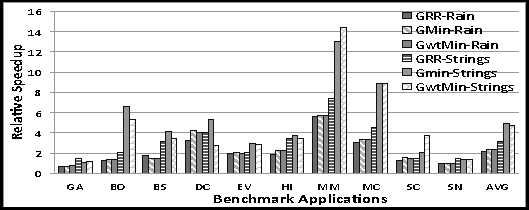
\includegraphics[width=3.2 in]{figures/strings_exp1.pdf}
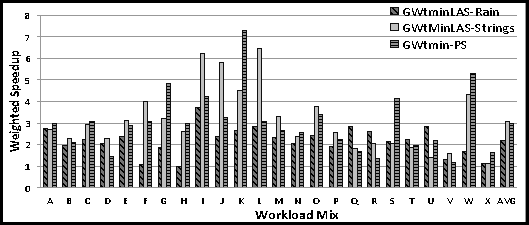
\includegraphics[width=0.75\textwidth,height=\textheight,keepaspectratio]{figures/strings_exp4.pdf}
\caption{Performance benefit of GPU scheduling. }
\label{fig:strings_exp4}
%\vspace{-1\baselineskip}
\end{figure}
\begin{figure}[h]
\centering
%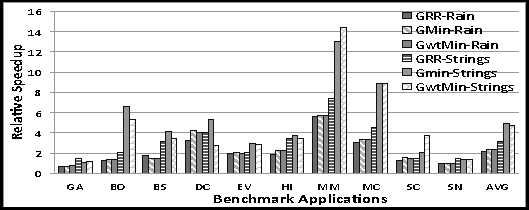
\includegraphics[width=3.2 in]{figures/strings_exp1.pdf}
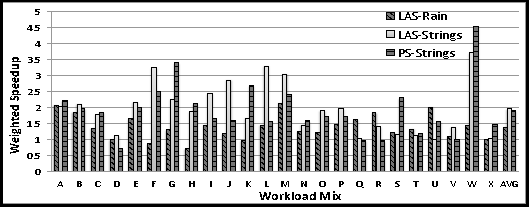
\includegraphics[width=0.75\textwidth,height=\textheight,keepaspectratio]{figures/strings_exp5.pdf}
\caption{Performance benefit of GPU scheduling policies.}
\label{fig:strings_exp5}
%\vspace{-1\baselineskip}
\end{figure}

\textit{2) Throughput Oriented Scheduler: } the baseline for this set of experiments is again the single node GRR policy, and scheduling policies are evaluated in combination with the best performing workload balancing policy from GPU sharing, i.e. GWtMin. As shown in Figure~\ref{fig:strings_exp4}, the average weighted speedup achieved with GWtMinLAS-Rain, GWtMinLAS-Strings, and GWtMin-PS is 2.18x, 3.10x, and 2.97x, respectively. The higher speedup achieved by LAS is because it greedily prioritizes the GPU requests that have shorter GPU episodes and have consumed less GPU time until the most recently completed scheduling epoch. This helps in completing the short running GPU jobs faster and thus increasing the overall system throughput. PS is a Strings-only scheduling policy specifically designed to leverage the concurrency opportunity exposed by CUDA streams and tries to keep all the hardware units in a GPU busy by favoring applications which are in different phases of their use of the GPU, to be active simultaneously. Although it slightly falls short in comparison to GWtMinLAS-Strings, by just 4\%, it does significantly better than   GWtMinLAS-Rain,   by   almost   27\%.   Therefore,   PS achieves  nearly  the  same  throughput  as  LAS  but  is  not  as unfair as LAS, which is an extremely greedy policy by definition and thus, might starve applications with relatively longer GPU episodes. The performance benefits shown in Figure~\ref{fig:strings_exp4} include the effect of both GPU sharing and device level GPU scheduling. To depict solely the benefits of GPU scheduling, Figure~\ref{fig:strings_exp5} compares the GPU scheduling policies with the baseline of GRR policy with four GPUs shared.  LAS-Rain, LAS-Strings and PS-Strings achieve 1.40x, 1.95x and 1.90x throughput improvement respectively over this baseline.

\textbf{Importance of Device-level Feedback.} Feedback-based policies are evaluated relative to the single node GRR policy. When the workload  balancer  receives  feedback  information from low-level GPU schedulers, it dynamically switches to the appropriate  feedback-based  load  balancing policy.  Figure~\ref{fig:strings_exp6} shows the weighted speedup achieved by two feedback-based policies, RTF and GUF, for both Rain and Strings. Average speedups attained are 2.22x, 2.51x, 3.23x, and 3.96x for RTF-Rain, GUF-Rain, RTF-Strings, and GUF-Strings, respectively. Compared to the highest speedup achieved by the previously discussed non-feedback based policy (GWtMinLAS-Strings), RTF-Strings and GUF-Strings achieve 4.5\% and 28\% improvements, respectively. Feedback-based policies outperform static workload balancing, because they make use of more detailed information about application characteristics. E.g., unlike GWtMin, which is a proactive scheduling policy that relies on static weights assigned to GPUs, RTF employs a reactive scheduling technique that uses the actual GPU-specific runtimes of applications to balance load. GUF outperforms RTF in the workload mix of applications that have widely contrasting GPU utilization, i.e., pairs with very high (DC, HT, MM and BO in Group A) and very low (Gaussian, SN and BS in Group B) GPU utilization, by not collocating multiple applications with high GPU utilization on the same GPU.
\begin{figure}[t]
\centering
%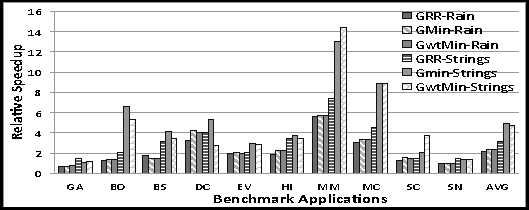
\includegraphics[width=3.2 in]{figures/strings_exp1.pdf}
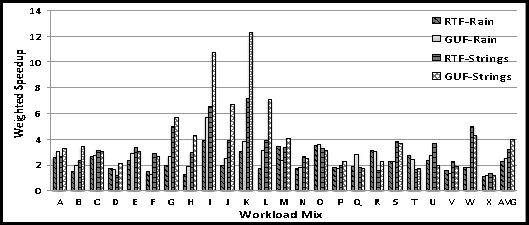
\includegraphics[width=0.75\textwidth,height=\textheight,keepaspectratio]{figures/strings_exp6.pdf}
\caption{Performance benefit of feedback-based load balancing.}
\label{fig:strings_exp6}
%\vspace{-1\baselineskip}
\end{figure}
\begin{figure}[t]
\centering
%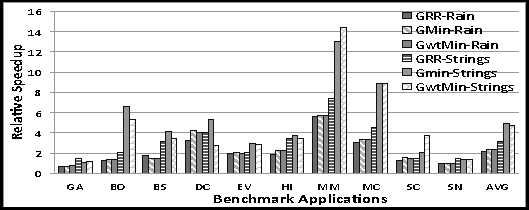
\includegraphics[width=3.2 in]{figures/strings_exp1.pdf}
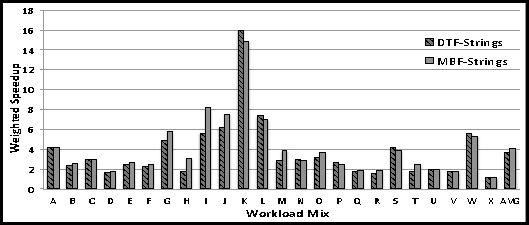
\includegraphics[width=0.75\textwidth,height=\textheight,keepaspectratio]{figures/strings_exp7.pdf}
\caption{Performance benefit of two Strings specific feedback-based load balancing policies.}
\label{fig:strings_exp7}
%\vspace{-1\baselineskip}
\end{figure}

Finally, we evaluate two Strings-specific feedback policies, DTF and MBF, which are designed to exploit the advantages offered by CUDA streams and context packing. As shown in Figure~\ref{fig:strings_exp7}, DTF and MBF achieve average speedups of 3.73x and 4.02x, respectively.  DTF performs best in a workload mix of applications with contrasting degrees of data transfer demands and GPU compute times, i.e., application pairs that have high GPU compute times (DC, EI, HT and MM in Group A) and high data transfer times (MC and SN in Group B). So, when one application is busy in data transfer to the device, the other can continue to use the device for computation. MBF, which is the best performing feedback-based policy, optimally performs in the workload mix of applications with sufficient asymmetry in their memory access behavior, i.e., application pairs with high GPU compute time but low memory bandwidth (EV and DC in Group A) and with high memory bandwidth (BS, HI and MC in Group B). This allows a higher degree of parallelism, by hiding the long memory latencies of memory-bound applications via a runtime switch to a compute-bound application. It is also important to note that by definition, MBF includes the benefits of both RTF and DTF, because the methodology to calculate the approximate memory bandwidth (the ratio of the total data accesses by its computation kernels to the total time spent in the GPU) includes both the data transfer and running time information of the application. This makes MBF perform better than RTF and GUF, across almost all workload mixes. MBF performs better than GWtMinLAS-Strings, RTF, and GUF by more than 30\%, 24\%, and 1.5\% respectively. Therefore, the maximum weighted speedup achieved across all the policies is 4.02x (MBF) relative to single node GRR policy, and 8.70x compared to the bare CUDA runtime.       

\textbf{Discussion. }Key insights from the experimental results in this section are the following. (1) GPU underutilization due to static collisions is avoided by making GPUs into explicitly scheduled entities, thus enabling the load balancing of GPU requests over an aggregated shared GPU pool (gPool). The outcome is an average speedup of up to 4.90x compared to the CUDA runtime. (2) GPU core idling can be reduced further by packing the GPU components of applications sharing a GPU into a single GPU context, causing improvements over schedulers without this ability of an average 2.10x for representative server workloads. (3) Fine-grain feedback from device-level scheduling to load balancing is important, as demonstrated by the fact that GMin performs better than GWtMin for some applications, despite the latter policy’s theoretical superiority. More generally, feedback policies outperform other workload balancing methods, achieving an average speedup of 8.70x. This is because they better understand application characteristics and can thus maximize GPU utilization by collocating applications with contrasting behavior in terms of data transfer and memory intensity. (4) Substantial advantages can be derived from collocating on the same device, streams of requests with likely unaligned peak performance demands, resulting in more uniform GPU usage patterns. Such uniformity is further encouraged by context packing and the consequent sharing of GPU context. (5) An important outcome of this work is that scheduling must go beyond considering GPU resources to also consider other schedulable device components, i.e., the GPU’s data movement engines. This is shown by the phase selection policy leveraging CUDA streams to keep all hardware units in a GPU busy. It achieves system throughput of 6.41x over the CUDA runtime, and it performs as well as the greedy, unfair LAS policy, but without compromising fairness.

\section{Related Work}
From the existing body of work on heterogeneous schedulers, StarPU~\cite{starpu} and Symphony~\cite{symphony} employ a dynamically learned performance model to decide which of the available resources to use, assuming optimized implementations of the same application targeted to different resources exist and can be dynamically dispatched to any one of them as needed. Previous work on interference-driven GPU resource management~\cite{phull} aims to provide better GPU utilization in heterogeneous clusters, by co-locating multiple jobs to share same GPU, respecting GPU memory constraints, but unlike Strings, which decouples the CPU and GPU components of a job and schedules them separately, ~\cite{phull} schedules both application components together on the same node, which might be restrictive. Further, Strings dynamically learns the application’s GPU characteristics, whereas ~\cite{phull} performs static profiling. 

Recent work~\cite{becchi} on managing GPU memory pressure arising from consolidating multiple applications on a single GPU is an interesting complement to our work. Similar middleware infrastructures have recently been proposed for other heterogeneous architectures like Intel’s Xeon Phi~\cite{phi}. By incorporating the virtual memory support of ~\cite{phi, becchi}, Strings can eliminate the assumption on the maximum rate of request arrivals in GPU servers. Gdev~\cite{gdev} implements open source versions of CUDA driver and the runtime library, using which, unlike [16] which presents its virtual memory abstraction at the runtime API level, it builds virtual memory support for GPUs inside the OS kernel. With the Gdev open source driver, both the context packer module and device-level scheduler of Strings can be pushed inside the OS kernel, eliminating runtime layer overheads. GEMTC middleware infrastructure~\cite{GPU43} implements a dynamic memory management system that efficiently allocates memory on the GPU. But unlike Strings, which is completely transparent to the applications, GEMTC exposes a set of new memory management APIs that require applications to be rewritten. Moreover, Strings supports management of heterogeneous multi-GPU resources on a single node which GEMTC infrastructure is yet to support.

In general, previous work on GPU virtualization GVim~\cite{gvim}, Pegasus~\cite{pegasus}, vCuda~\cite{vcuda}, rCuda~\cite{rcuda}, gVirtus~\cite{gvirtus} make the GPUs visible from within the virtual machine. GVim and Pegasus both do QoS-aware scheduling by using a working queue per GPU, but they do not address the problem of scheduling GPU requests across multiple GPUs within a node or across multiple nodes in a cluster. Pegasus also explores the co-scheduling of GPU request with corresponding VCPUs. This can be combined with our Strings infrastructure by gang scheduling decoupled application's CPU and GPU components. vCuda and rCuda leverage the multiplexing mechanism of the bare CUDA runtime for GPU sharing, but they don't look into scheduling policies targeting various resource management goals. 

\section{Chapter Summary}
This chapter presents the Strings scheduler and scheduling policies for GPUs as first class schedulable entities in high-end cloud services. Decomposing the scheduling problem into a combination of workload balancing and device-level scheduling, Strings contributes scheduling policies that explicitly consider data movement to/from accelerators, methods that dynamically encapsulate the GPU contexts of multiple applications into a single umbrella context to achieve high GPU utilization and minimize context switching overhead, and support that makes possible the runtime switching of policies based on device-level scheduler feedback. Novel scheduling policies developed with Strings include (i) a Phase Selection (PS) policy that aims to keep all of a GPU’s hardware units busy by smartly picking and simultaneously running applications operating in different phases of their use of the GPU, (ii) advanced feedback-based policies like DTF and MBF that exploit the advantages offered by CUDA streams and context packing, by collocating applications with contrasting behavior, in terms of data transfer and memory intensity, to achieve extreme performance benefits, (iii) a throughput oriented greedy but highly unfair LAS policy favoring jobs with least-attained levels of GPU service, and (iv) history-based fairshare scheduling that improved fairness in GPU usage for multi-tenant applications.

Extensive experimental evaluations across a wide variety of workloads and system configurations shows Strings to achieve speedups of up to \textbf{4.90x} and \textbf{2.07x} on a single node compared to the CUDA runtime and over our own previous GPU scheduling work, Rain, respectively. Averaged over 24 pairs of short and long running workload mix, Strings achieve a weighted speedup of up to \textbf{8.70x }and \textbf{13\%} improvements in fairness over the CUDA runtime.

Our future work will consider dynamic opportunities and tradeoffs in mapping executions to either GPUs or CPUs, using runtime methods for binary translation~\cite{ocelot}. Also interesting is further exploration of the effects of data movement on program performance and consequent changes in scheduling policies, first for discrete vs. integrated GPUs and second considering GPU multi-tenancy.
